\documentclass[a4paper,11pt]{article}
\usepackage[utf8]{inputenc}
\usepackage[top=3cm,left=2cm,right=2cm,bottom=2cm]{geometry}
\usepackage{graphicx}
\usepackage[usenames,dvipsnames]{xcolor}
\usepackage{multicol}
\usepackage{wrapfig}
\usepackage[french]{babel}
\usepackage{listings}
\usepackage{datetime}
\usepackage[cache=false]{minted}
\usepackage{caption}
\title{Online Platform for Machine Learning}
\author{\textbf{DEMBELE} Mama, \textbf{DAOUMA} Zakaria, \textbf{N'DIAYE} Laity}
\date{\today}
\begin{document}
\makeatletter
  \begin{titlepage}
   \begin{flushleft}
        
\includegraphics[scale=0.2, width=4cm]{logo.png}
     \end{flushleft}
       \hfill
     \vspace{2em}
   \begin{center}
   {\large \textsc{Polytech'Marseille}}
  \end{center}
  \vspace{1em}
   \begin{center}
     \Large\textbf{\textit{Rapport de projet}}\\
     \vspace{1em}
    {\large\@date\\}
    \vspace{3em}
       {\LARGE \textcolor{blue}{\textbf{\textit{\@title}}}} \\
    \vspace{3em}
        {\large \@author}\\
        \vspace{1em}
       Informatique 4ème année.
   \end{center}
\vspace{2cm}
\begin{flushleft}
\em{Tuteur de projet : Agus Budi Raharjo}
\end{flushleft}
 \vfill
 \end{titlepage}
\makeatother
\renewcommand{\contentsname}{Sommaire}
\renewcommand{\thesection}{\arabic{section}}
\setcounter{secnumdepth}{4}
\setcounter{tocdepth}{4}
\tableofcontents
\newpage
\section{Introduction}
Ce document a pour but de rendre compte du travail effectué dans le cadre du projet de 4ème année de l’option InSi. Notre sujet principal est le développement d’une plateforme web permettant à toute personne de pouvoir comparer l'efficacité de certains algorithmes  de Machine Learning en les appliquant sur des données concrètes.
Le choix de ce sujet n’est pas anodin car Machine Learning est la nouvelle tendance.
Son but est de permettre à la machine d’apprendre par elle-même, ce qui peut s’avérer très bénéfique dans beaucoup de domaines.
En choisissant ce sujet nous espérons approfondir nos connaissances dans ce domaine et pouvoir l’appliquer sur des exemples concrets.

Nous présenterons d’abord les architectures matérielle et logicielle de plateforme, basées sur nos analyses préalables.
Ce sera l’occasion de comprendre comment fonctionne le Machine Learning, et de connaître quels sont les dispositifs matériels, les langages de programmation et les algorithmes qui s’offrent à nous.

Dans la seconde partie, nous parlerons de la mise en place de la plateforme sur le web
et de l’utilisation par un utilisateur lambda. Ensuite, nous montrerons les résultats obtenus.
On retrouvera donc une page concernant la gestion de projet, qui explique notre planning, et nos stratégies de
développement..

Enfin, la dernière partie permet de se rendre compte de tout ce que nous avons pu apprendre au cours
de ce projet et réfère les différents problèmes auxquels nous avons dû faire face. Elle a, elle aussi,
un réel intérêt puisque nous avons fait en sorte de décrire précisément les étapes difficil
es et nos démarches
pour les surmonter, et donc peut servir d’aide pour un futur projet ainsi que le témoignage de notre progression.

\section{Réalisation}
    \subsection{Description de l'application}
Dans ce chapitre on va décrire comment fonctionne notre plateforme.\\
Ce projet ayant comme sujet la création d’une plateforme de Machine learning, il est d’abord nécessaire de la présenter.\\
Notre plateforme permet à tout utilisateur de pouvoir observer la magie du machine learning en téléchargeant des fichiers de données et en choisissant des algorithmes
à appliquer.\\\\
\textbf{Comment ça marche ?}\\

\includegraphics[width=17cm, height=10cm]{homePage.png}\\\\
L’utilisateur pourra, en cliquant sur le lien \og Get started \fg( voir figure ci-dessus), ajouter ses fichiers de données d’apprentissages et/ou de tests ainsi que choisir des algorithmes et des méthodes de validation des données ( cross validation par exemple ) comme indiqué sur l’image ci-dessous :\\\\

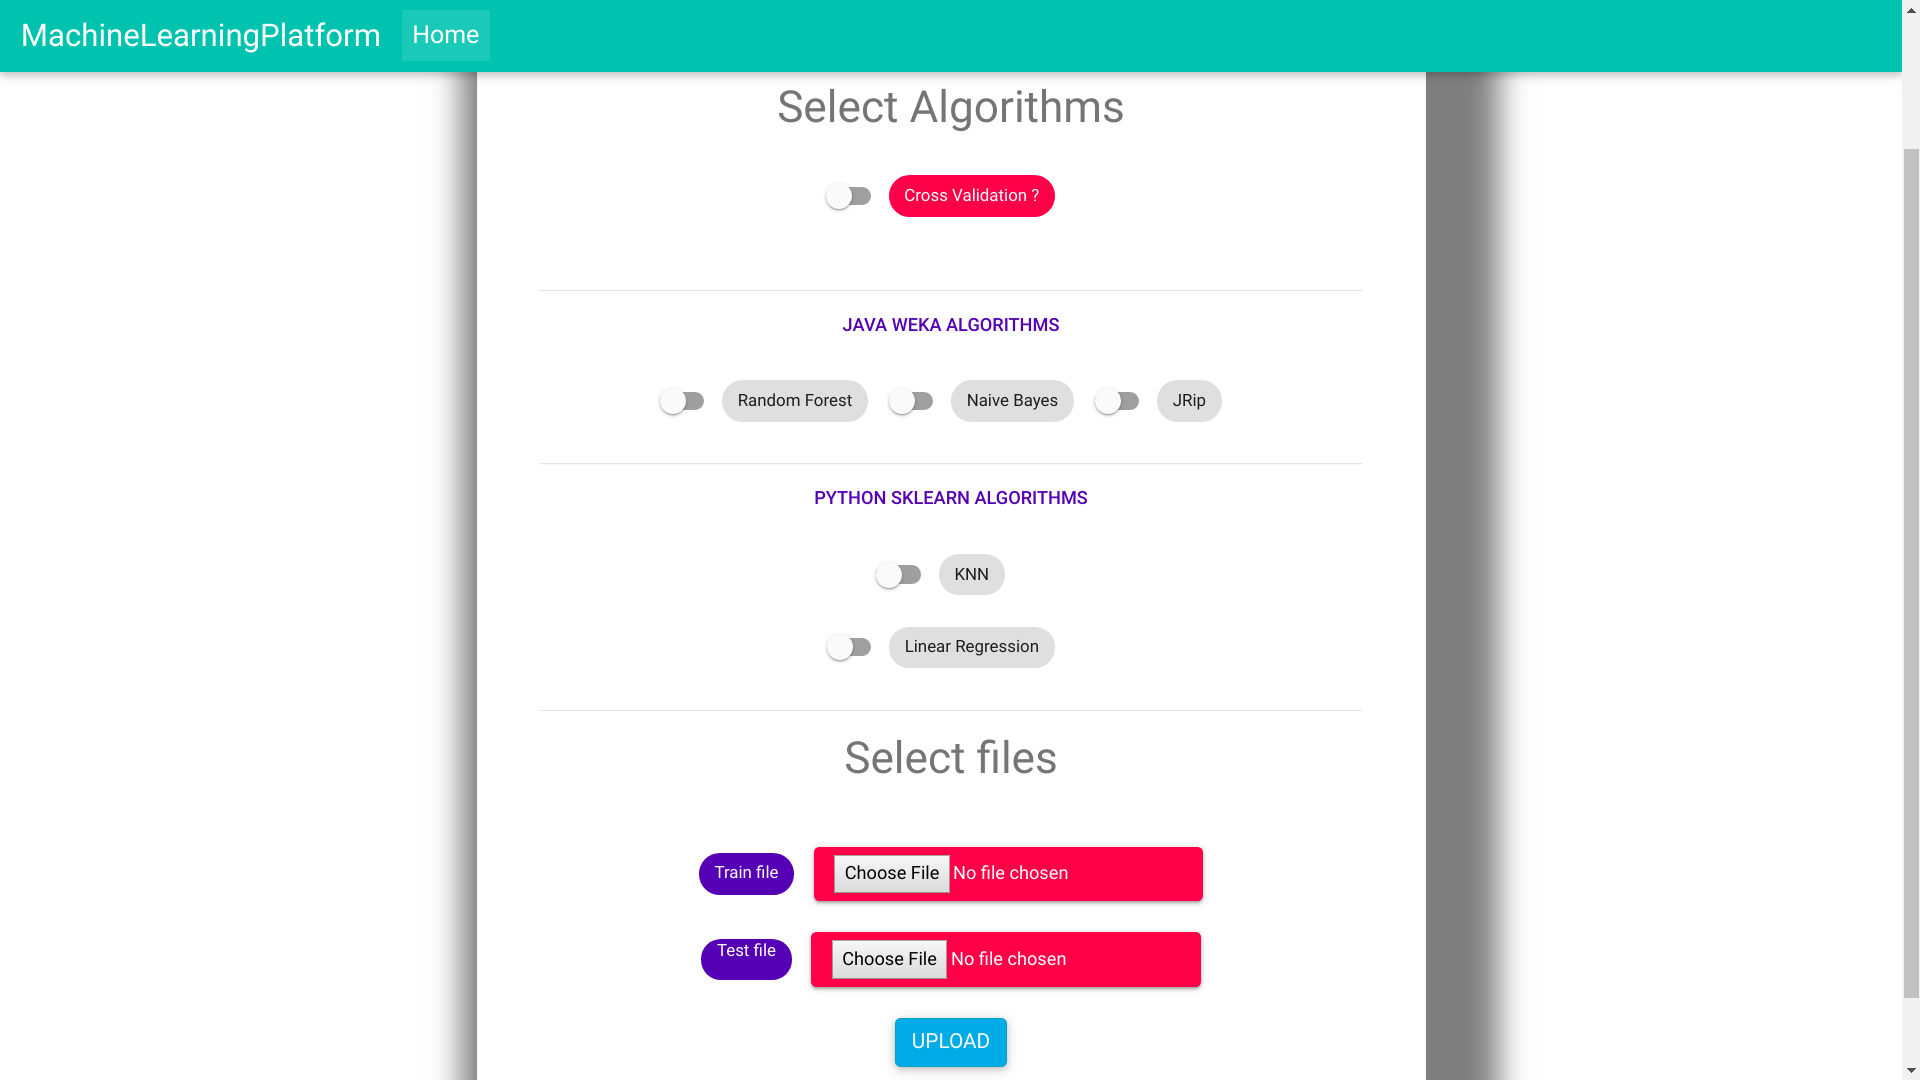
\includegraphics[width=17cm, height=10cm]{upload.png}\\\\
Il peut également choisir la cross validation ( qui lui permettra de ne mettre que les données d’entraînement ) :\\\\

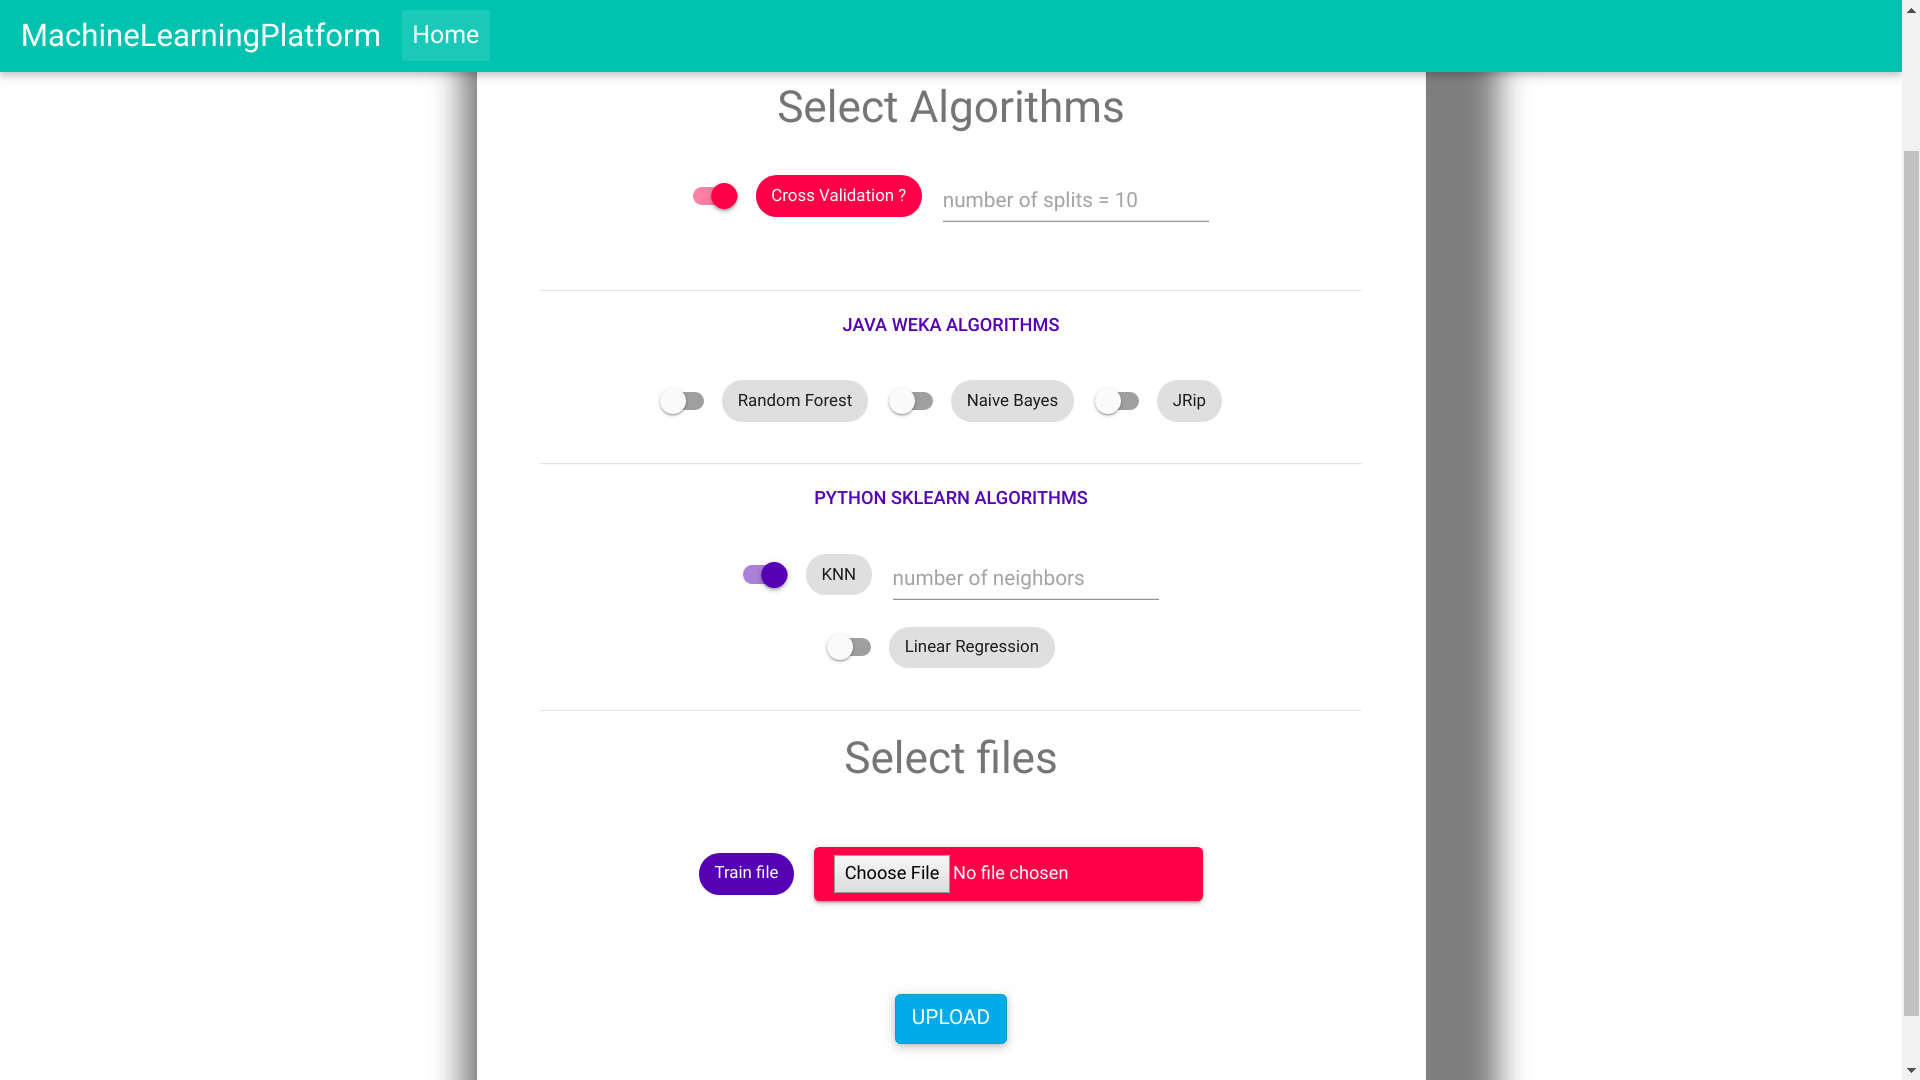
\includegraphics[width=17cm, height=10cm]{upload_cv_knn.png}\\\\

Après quoi l'utilisateur pourra , en cliquant sur le bouton \og upload \fg, voir le graphique de comparaison entre les différents algorithmes comme sur l'image ci-dessous :\\\\

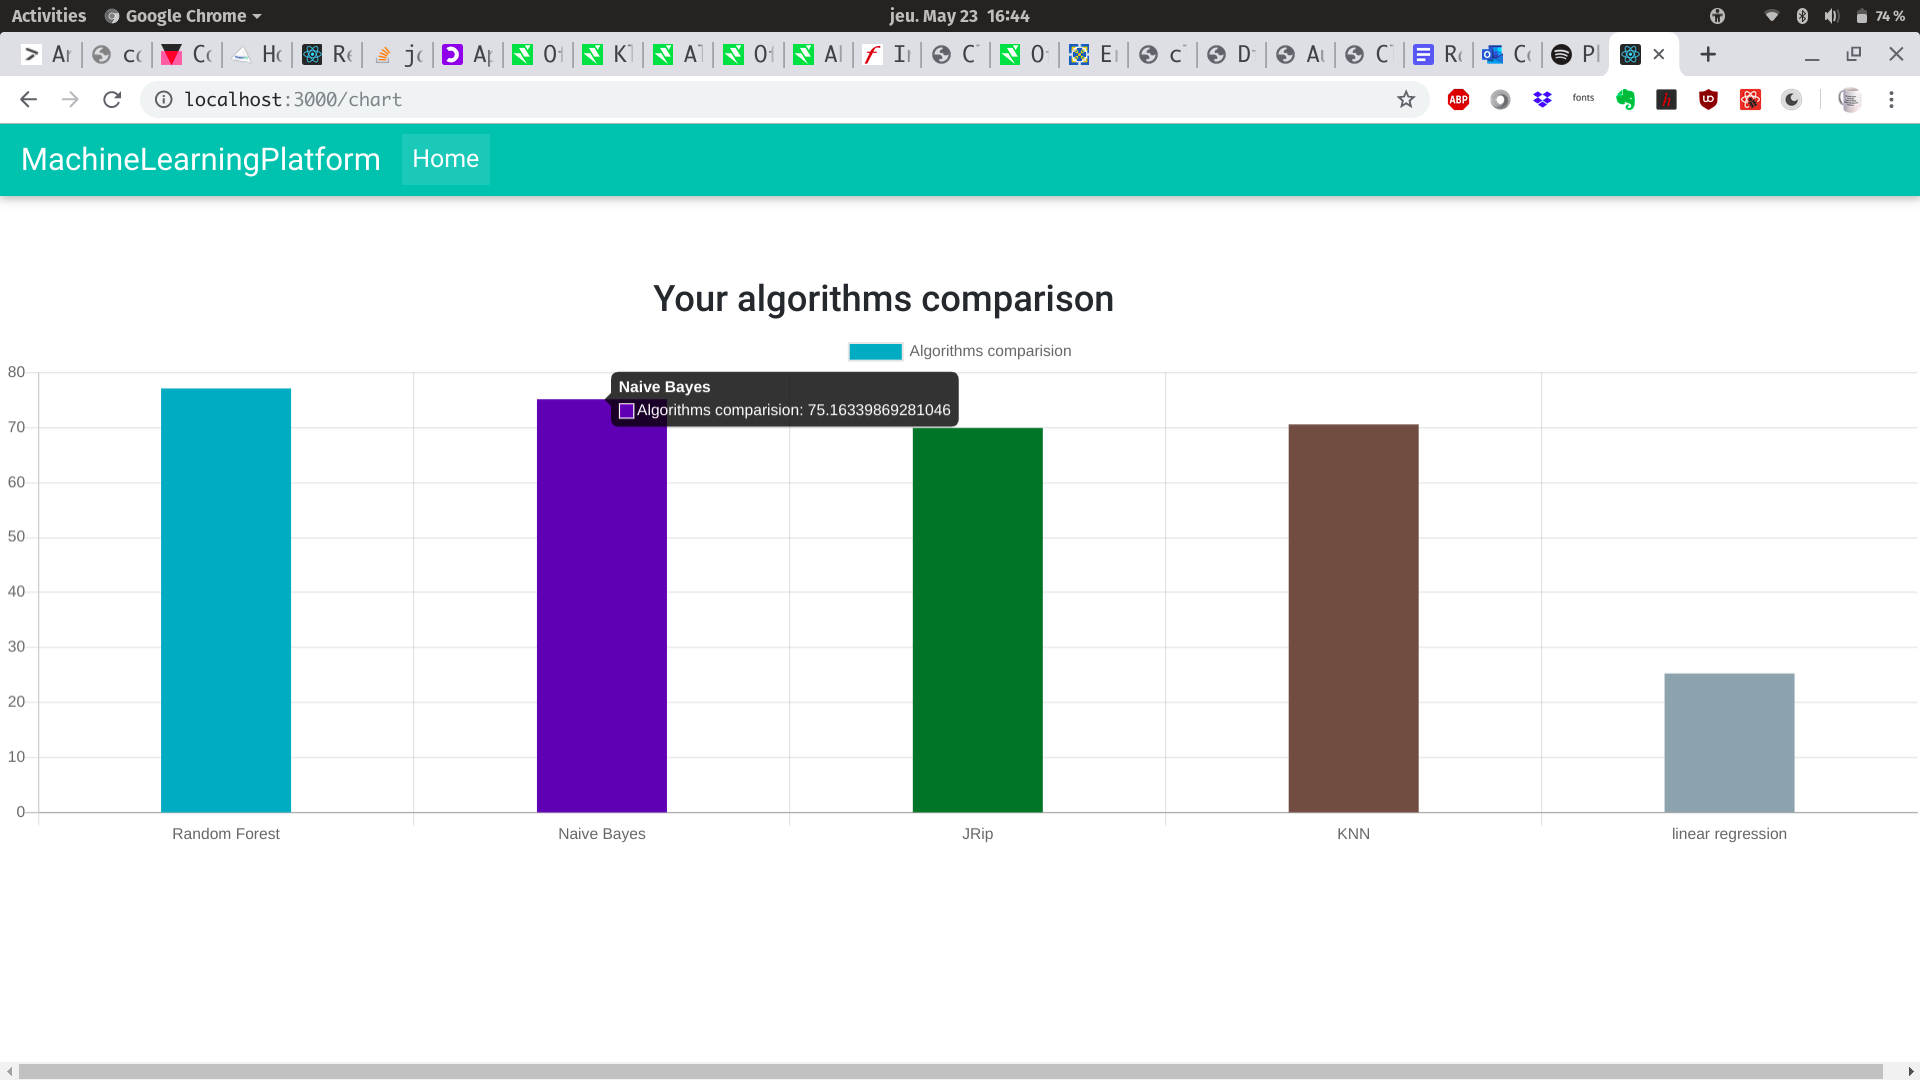
\includegraphics[width=17cm, height=10cm]{algoComparison.png}\\\\

\textbf{Qu'est ce que Machine Learning ?}\\\\

Machine Learning est une branche de l'intelligence artificielle permettant aux ordinateurs d'apprendre sans avoir été programmés explicitement à cet effet.
Pour apprendre et se développer, les ordinateurs ont toutefois besoin de données à analyser et sur lesquelles s'entraîner.
Il s'agit d'une science moderne permettant de découvrir des patterns et d'effectuer des prédictions
à partir de données en se basant sur des statistiques, sur du forage de données, sur
les reconnaissances de patterns et sur les analyses prédictives:

\begin{itemize}
    \item Nous avons donc créée une plateforme à l’aide de
     laquelle, un utilisateur peut charger ses données
    et choisir parmi un ou plusieurs algorithmes qui affichera des résultats et montrera l’efficacité de ceux-ci.

    \item Ce dernier peut également opter pour la cross validation afin que la répartition des données soit faite de manière aléatoire.

\end{itemize}



\subsection{Outils utilisés}
Pour ce projet on a utilisé beaucoup d'outils actuels de développement Web et de Machine Learning :

\begin{itemize}
    \item Certains algorithmes ont été développés en utilisant la bibliothèque \emph{Weka de Java}
    qui est une bibliothèque très utilisée et facile à prendre en main pour le Machine Learning.

    \item D'autres ont été développés en utilisant la bibliothèque \emph{Scikit-learn de Python}
    qui est la bibliothèque par excellence quand on commence le Machine Learning.

    \item L'interface utilisateur de l’application ( frontend ) a été développée en utilisant \emph{React} qui est une bibliothèque Javascript développée par Facebook pour développer facilement et rapidement des applications web monopage.
    Le design utilise \emph{Material-ui} et \emph{Bootstrap} qui sont des framework populaires \emph{CSS} de design.
    Les histogrammes de résultat de comparaison des algorithmes sont modélisés par la bibliothèque \emph{Javascript Chart.js} qui permet d’afficher des graphiques dans une page web.

    \item Les API REST sont développées en Python avec le framework Flask et Java avec le framework SpringBoot

    \item Tous les développements ont été faits sur Linux en utilisant l’\emph{IDE IntelliJ}

\end{itemize}

    \subsection{Environnement}
La plateforme est développée uniquement pour les utilisateurs web c’est-à-dire qu’il n’y a pas d’application mobile.
Tous les développements ont été faits sur nos machines chez nous en privilégiant le travail en équipe. Donc la mise en place des créneaux réguliers de travail était nécéssaire.
\subsubsection{La répartition et l'ordonnancement des tâches}

Comme dans tout projet, l'organisation peut souvent s'avérer très compliquée
mais ayant l'avantage d'être moins nombreux, on est arrivés à s'organiser facilement:

\begin{itemize}
    \item Analyse matérielle et logicielle de la plateforme	  (Laity, Zakaria et Mama)

    \item Mise en place du Back-end					(Mama et Zakaria)

    \item Développement algorithmes Python et test  	 	(Zakaria)

    \item Développement algorithmes Java et test  			(Mama)

    \item Elaboration du Front End : mise en place de l’IHM	(Laity)

    \item Implémentation des nouvelles fonctions			(Zakaria et Mama)

    \item Préparation de la soutenance + rédaction rapport	 (Laity, Mama et Zakaria)

\end{itemize}

Durant la totalité du projet, nous avons essayé de jouer le plus possible le jeu de l’ingénieur et du client ou du chef de projet en tenant informé notre tuteur de projet des dernières avancées (client) et en lui demandant des conseils lorsqu’on avait des problèmes (chef de projet).

\subsection{Architecture}
Ici nous  allons développer l’architecture globale de notre application.
Toutes nos API (Spring-Boot/java et Flask/Python ) utilisent l’architecture MVC (Model - View - Controller)
qui est une architecture de développement d’applications très utilisée pour une meilleure organisation et lisibilité.
Pour l’interface utilisateur, React étant une bibliothèque et n’imposant pas d’architecture particulière,
on a décidé de mettre en place une architecture type microservices c’est-à-dire chaque composant permet de
rendre un service particulier comme la navigation qui est gérée par un service particulier,
l’upload des fichiers et envoi des fichiers etc.\\
Vous pouvez observer l’architecture globale sur l’image ci-dessous :

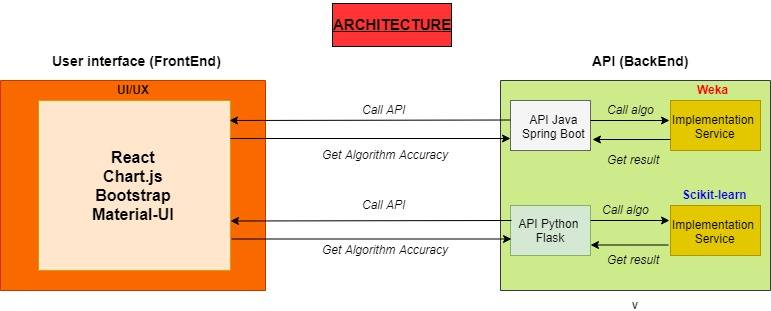
\includegraphics[width=14cm, height=6cm]{archi.jpg}\\


\subsection{Résultats obténus}

Après à peu près 3 mois de travail on obtient des résultats escomptés.
Le but premier a été bien atteint. Cépendant il reste encore des améliorations/ajouts à faire.
On a bien une application web qui permet de faire des appels distants à des API et qui permet de bien afficher
des graphiques comparant ces algorithmes.

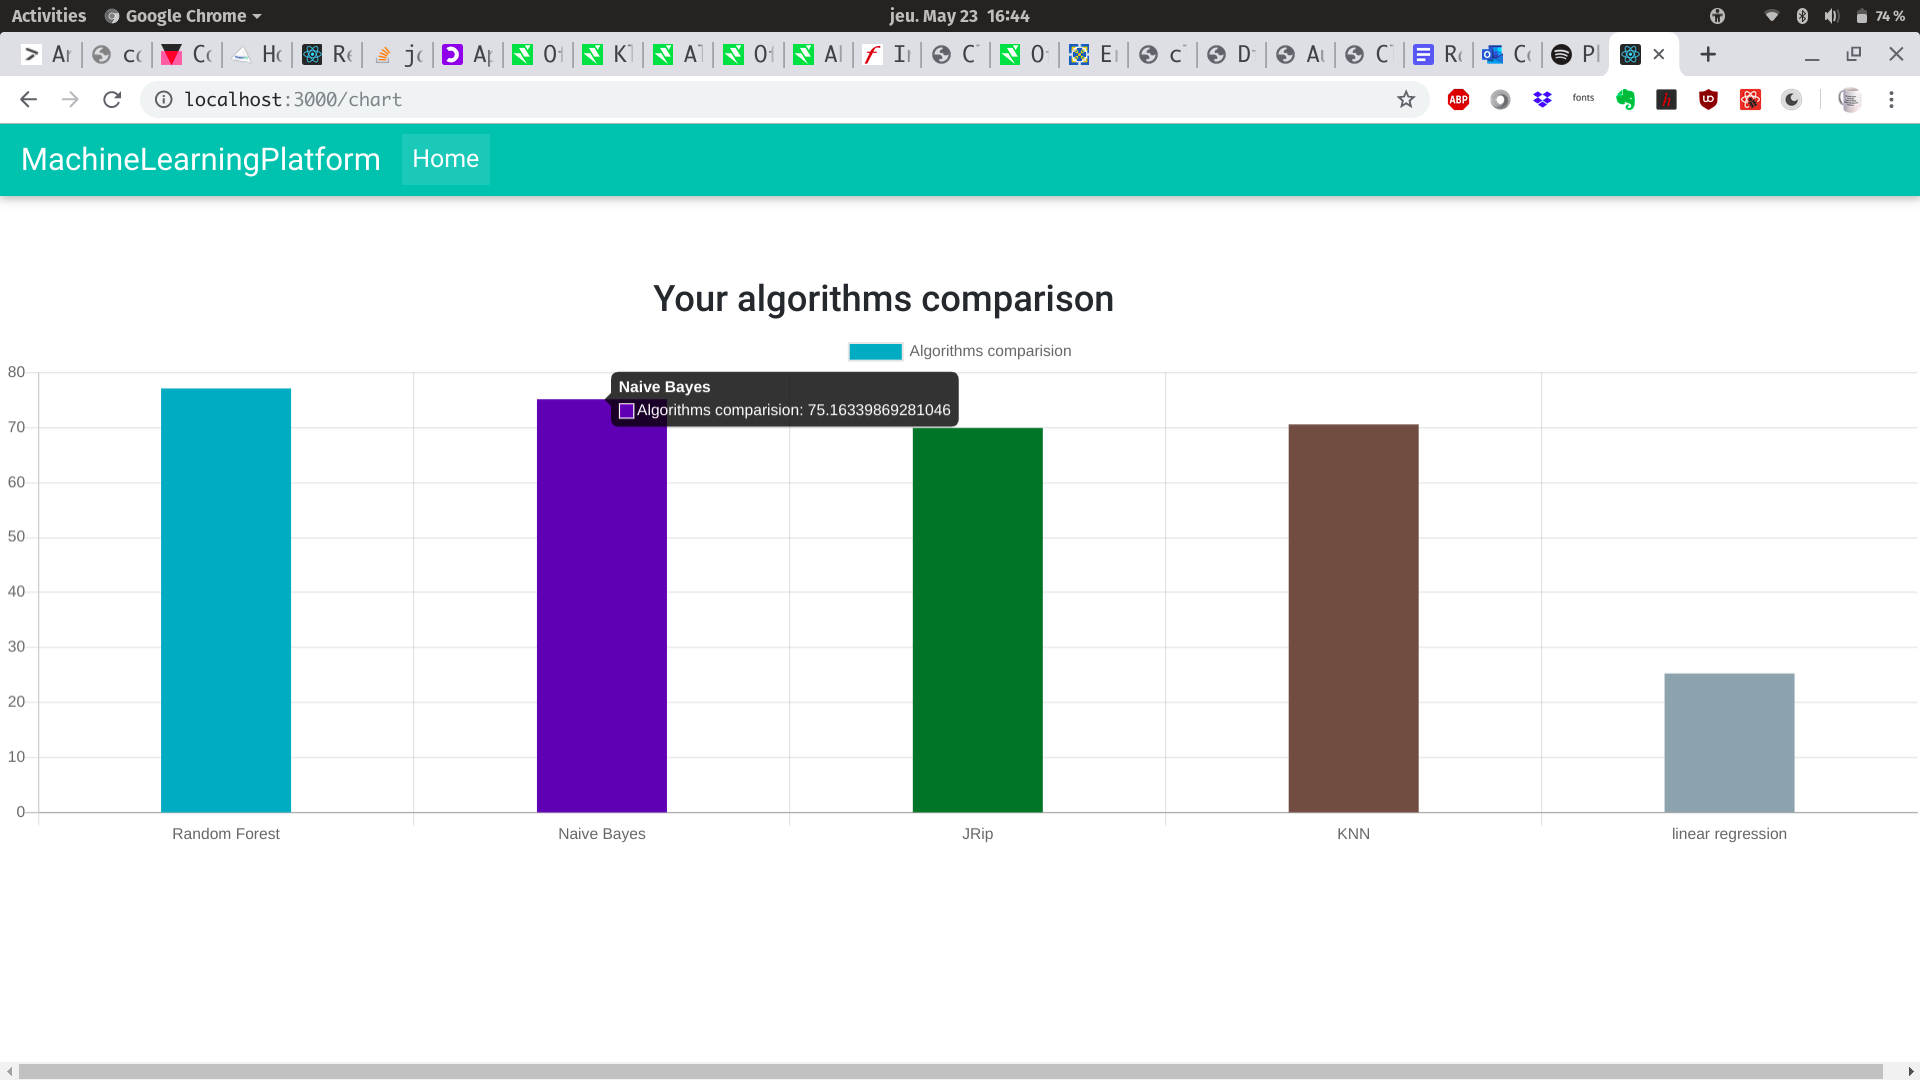
\includegraphics[width=17cm, height=10cm]{algoComparison.png}\\

    \section{Bilan du projet}
\subsection{Points positifs}
Lors de ce projet nous avons pu comprendre à quel point le travail de groupe et la rigueur sont importantes dans la réalisation dans un tel projet.\\
En effet un retard dans la réalisation des tâches de l’un des membres peut impacter
le travail de l’autre donc la communication entre les membres du groupe est primordiale.\\
Ce projet nous a permis d'approfondir nos connaissances du machine learning
(utilisation des bibliothèques populaires, implémentation des algorithmes etc.) et du développement
d'application web( séparation de l'interface utilisateur du serveur et leur communication via des API REST).

\subsection{Points à améliorer}
\begin{itemize}
    \item Ajout de plusieurs algorithmes pour élargir les possibilités

    \item Affichage d'autres caractéristiques des algorithmes.

    \item Plus de possibilités de manipulation des graphiques par l’utilisateur (masquer/démasquer certains graphiques)

\end{itemize}

\subsection{Conclusion}
Ce projet nous a d'abord permis de nous familiariser avec une plateforme web et les algorithmes
de programmation en Machine Learning. C'est un domaine qui est assez multidisciplinaire puisqu'il
englobe des notions de développement web, de réseaux, de programmation, de graphisme d'application.

    \section{Annexe}
\subsection{Code source}
    
    \begin{itemize}
        \item Frontend (l'interface utilisateur)
            \begin{itemize}

                \item \textbf{Nav.js}
\begin{minted}[breaklines]{python}
    import React, { Component } from 'react';
    import { Link } from "react-router-dom";
    import {Typography} from "@material-ui/core";

    /**
    * La page de navigation
    */
    export default class Nav extends Component{

        render() {
            return(
                <nav className="mb-1 navbar fixed-top navbar-expand-lg navbar-dark default-color">
                    <a className="navbar-brand" href="/">
                        <Typography variant="display1" style={{fontSize: '1.2em', color: 'white'}}>
                            MachineLearningPlatform
                        </Typography></a>
                    <button className="navbar-toggler" type="button" data-toggle="collapse" data-target="#navbarSupportedContent-333"
                        aria-controls="navbarSupportedContent-333" aria-expanded="false" aria-label="Toggle navigation">
                        <span className="navbar-toggler-icon"></span>
                    </button>
                    <div className="collapse navbar-collapse" id="navbarSupportedContent-333">
                        <ul className="navbar-nav mr-auto">
                            <li className="nav-item active">
                                <Link className="nav-link" to="/">
                                    <Typography variant="display1" style={{fontSize: '1.2em', color: 'white'}}>Home</Typography>
                                </Link>
                            </li>
                        </ul>
                    </div>
                </nav>
            );
        }

    }

\end{minted}
\item \textbf{Home.js}
\begin{minted}[breaklines]{python}
import React from 'react';
import img from '../assets/img/ml.png';
import '../styles/styles.css';
import { Link } from "react-router-dom";
import {Button, Typography} from "@material-ui/core";

/**
* La classe générant la page d'acceuil
*/
export default class Home extends React.Component{

    render() {
        return (
            <div>
                <div style={ style } className="homeDiv"></div>
                <div style={{ color: 'white', position: 'relative', top: 150, left: 150}} className="h2 col-md-6">
                    <Typography style={{color: 'white'}} variant="display1">Welcome to our Machine Learning Platform,</Typography>
                </div>
                <div style={{ color: 'white', position: 'relative', top: 170, left: 150}} className="h2 col-md-6">
                    <Typography style={{color: 'white'}} variant="display1">upload your files and see the magic worked
                        with our algorithms.</Typography>
                </div>
                <div style={{ position: 'relative', top: 190, left: 150}} className="col-md-3">
                    <Link to="/upload" style={{textDecoration: 'none'}}>
                        <Button variant="contained" color="secondary">
                            Get started
                        </Button>
                    </Link>
                </div>
            </div>
        );
    }

}

const style = {
    position: 'absolute',
    height: "100%",
    width: "100%",
    backgroundImage: `url(${img})`,
}
\end{minted}
\item \textbf{Upload.js}
\begin{minted}[breaklines]{python}
import React, { Component } from 'react';
import axios from 'axios';
import { Route } from 'react-router-dom';
import FormControlLabel from "@material-ui/core/FormControlLabel";
import Switch from "@material-ui/core/Switch";
import Button from "@material-ui/core/Button";
import {Input, Typography} from "@material-ui/core";
import Chip from "@material-ui/core/Chip";
import CircularProgress from "@material-ui/core/CircularProgress";

/**
* La classe gérant l'upload des fichiers
* Elle permet de récupérer les fichiers et
* de les envoyer aux serveurs
*/
export default class Upload extends Component{

    constructor(props){
        super(props);

        //Définition des variables d'état.
        this.state = {
            train: null,
            test: null,
            testShow: 'inline-block',
            rf: false,
            nb: false,
            jr: false,
            knn: false,
            lr: false,
            cv: false,
            nbSplits: '',
            nbSplitsShow: 'none',
            neighborsShow: 'none',
            neighbors : '',
            jRedirect: false,
            pyRedirect: false,
            error: '',
            pyLoading: false,
            jLoading: false
        };

        this.onSubmit = this.onSubmit.bind(this);
        this.java = this.java.bind(this);
        this.python = this.python.bind(this);
        this.upload = this.upload.bind(this);
        this.toggleCV = this.toggleCV.bind(this);
        this.toggleKNN = this.toggleKNN.bind(this);
    }


    /**
    * Cette fonction renvoie vraie quand tous les algorithmes de java
    * sont sélectionnés
    * @returns {boolean}
    */
    java = () => {
        return this.state.nb || this.state.jr || this.state.rf;
    };

    /**
    * La même chose pour les algos de python.
    * @returns {boolean|*}
    */
    python = () => {
        return this.state.lr || this.state.knn;
    };

    /**
    * La fonction faisant l'upload proprément dit
    * @param serverAddress l'adresse du serveur
    * @param data les données à envoyer
    * @param server le type de serveur (java ou python)
    */
    upload = (serverAddress, data, server) => {
        if(server === 'java') {
            //On met l'état jloading à true pour dire que on est entrain de faire appel au serveur
            //java
            this.setState({jLoading: true});
            axios.post(serverAddress, data)
            .then(res => {
                //Dès qu'on reçoit la réponse l'état jloading dévient false.
                this.setState({jLoading: false});
                    localStorage.setItem('data', JSON.stringify(res.data));
                    this.setState({
                    jRedirect: true,
                });
            })
            .catch(error => {
                this.setState({jLoading: false});
                this.setState({
                    error: <div className="alert alert-danger" role="alert">Problème au niveau du serveur java</div>
                });
            });
        }else{
            this.setState({pyLoading: true});
            axios.post(serverAddress, data)
                .then(res => {
                    this.setState({pyLoading: false});
                    localStorage.setItem('data2', JSON.stringify(res.data));
                    this.setState({
                    pyRedirect: true
                });
            })
            .catch(error => {
                this.setState({pyLoading: false});
                this.setState({
                    error: <div className="alert alert-danger" role="alert">Problème au niveau du serveur Python</div>
                });
            });
        }

    };

    /**
    * Cette fonction est appélée dès qu'on clique sur le bouton upload
    * qui va faire appel à la fonction upload précedemment définie.
    * @param e
    */
    onSubmit(e) {
        e.preventDefault();

        //Validation de données
        if(this.state.train === null || (!this.state.cv && this.state.test === null))
            this.setState({
                error: <div className="alert alert-danger" role="alert">Please select your train and test file</div>
            });
        else if(!this.state.nb && !this.state.rf && !this.state.jr && !this.state.knn && !this.state.lr )
            this.setState({
                    error: <div className="alert alert-danger" role="alert">Please select at least one algorithm</div>
            });
        else {

            let data1 = new FormData();
            let data2 = new FormData();
            data1.append('train', this.state.train);
            data1.append('test', this.state.test);
            data2.append('train', this.state.train);
            data2.append('test', this.state.test);

            data1.append('rf', this.state.rf);
            data1.append('nb', this.state.nb);
            data1.append('jr', this.state.jr);
            data1.append('cv', this.state.cv);
            if(this.state.nbSplits !== '')
                data1.append("nbSplits", this.state.nbSplits);

            data2.append('lr', this.state.lr);
            data2.append('knn', this.state.knn);
            data2.append('cv', this.state.cv);
            if(this.state.cv)
                data2.append("nbSplits", this.state.nbSplits);
            if(this.state.knn)
                data2.append("neighbors", this.state.neighbors);

            //Si on a que des algos de java qui sont sélectionnés
            if (this.java() && !this.python()) {
                this.setState({pyRedirect: true});
                this.upload('http://localhost:8080/upload', data1, 'java');

            // que les algos de python
            } else if (!this.java() && this.python()) {
                this.upload('http://localhost:5000/upload', data2, 'python');
                this.setState({jRedirect: true});

            //au moins 1 algo sélectionné des deux côtés.
            } else {
                this.upload('http://localhost:5000/upload', data2, 'python');
                this.upload('http://localhost:8080/upload', data1, 'java');
            }
        }

    }

    //Dès que le composant est monté, on supprime les deux cookies qui ont
    //été mis en place entre l'upload et le composant qui affiche les graphiques.
    //pour éviter des affichages érronés.
    componentDidMount() {
        localStorage.removeItem('data');
        localStorage.removeItem('data2');
    }

    /**
    * Quand on clique sur le switch de cross validation
    * cette fontion est appelée pour faire apparaître la case ou mettre le nombre
    * de splits et cacher l'input de fichier test
    * @param e
    */
    toggleCV = (e) => {
        this.setState({cv: e.target.checked});
        if (e.target.checked)
            this.setState({nbSplitsShow: 'inline-block', testShow : 'none'});
        else
            this.setState({nbSplitsShow: 'none', testShow: 'inline-block'});
    };

    //Pareil ici que toggleCV
    toggleKNN = (e) => {
        this.setState({knn: e.target.checked});
        if (e.target.checked)
            this.setState({neighborsShow: 'inline-block'});
        else
            this.setState({neighborsShow: 'none'});
    };

    /**
    * La fonction qui est appelée quand le composé est monté dans le DOM
    * si au moins un des états jloading ou pyloading vaut vrai on affiche plutot
    * un progress bar de type circulaire.
    * @returns {*}
    */
    render() {
        return(
        this.state.pyLoading || this.state.jLoading ?
            <div className="row text-center" style={{ marginTop : '300px'}}>
            <div className="col-md-5"></div>
                <div className="col-md-3">
                    <CircularProgress color="secondary" style={{width: '70px'}}/>
                <Typography variant="title">Please wait</Typography>
                </div>
            </div> :
            this.state.jRedirect && this.state.pyRedirect ?
                <Route render={({ history }) => history.push("/chart")  }/> :

        <div className="container">
            <div className="row" style={{marginTop: '70px'}}>
            <div className="col-md-3"></div>
            <div className="col-md-6">
                {this.state.error}
            </div>
            </div>
            <div className="row" style={{marginTop: '70px'}}>
                <div className="col-md-2"></div>
                <div className="col-md-8">
                <form
                    className="text-center border border-light p-5"
                    onSubmit={this.onSubmit}
                    style={{boxShadow: '22px 12px 22px 34px gray'}}
            >
                <Typography variant="display1">Select Algorithms</Typography>
            <br/>
            <div className="col">
                <FormControlLabel
                    control={
                        <Switch
                            onChange={this.toggleCV}
                            value="cv"
                            color="secondary"
                        />
                    }
                    label={<Chip label="Cross Validation ?" color="secondary"/> }
                />
                    <Input
                        placeholder="number of splits = 10"
                        style={{ display: this.state.nbSplitsShow}}
                        onChange={(e) => this.setState({nbSplits : e.target.value})}
                    />
                </div>
                <br/>
                <hr/>
            <div className="col">
                <Typography variant="button" color="primary">Java weka algorithms</Typography>
            </div>
            <br/>
            <FormControlLabel
                control={
                    <Switch
                        onChange={(e) => this.setState({rf: e.target.checked})}
                        value="rf"
                        color="primary"
                    />
                }
                    label={<Chip label="Random Forest" color="default"/> }
                />
            <FormControlLabel
                control={
                    <Switch
                        onChange={(e) => this.setState({nb: e.target.checked})}
                        value="nb"
                        color="primary"
                    />
                }
                    label={<Chip label="Naive Bayes" color="default"/> }
                />
            <FormControlLabel
                control={
                    <Switch
                    onChange={(e) => this.setState({jr: e.target.checked})}
                    value="jr"
                    color="primary"
                />
                }
                label={<Chip label="JRip" color="default"/> }
            />
            <br/>
            <hr/>
            <div className="col">
                <Typography variant="button" color="primary">Python SKlearn algorithms</Typography>
            </div>
            <br/>
            <div className="col">
                <FormControlLabel
                control={
                    <Switch
                        onChange={this.toggleKNN}
                        value="knn"
                        color="primary"
                    />
                    }
                    label={<Chip label="KNN" color="default"/> }
                />
                <Input
                    placeholder="number of neighbors"
                    style={{ display: this.state.neighborsShow }}
                    onChange={(e) => this.setState({neighbors : e.target.value})}
                />
            </div>
                <FormControlLabel
                control={
                    <Switch
                        onChange={(e) => this.setState({lr: e.target.checked})}
                        value="lr"
                        color="primary"
                    />
                    }
                    label={<Chip label="Linear Regression" color="default"/> }
                />
                <hr/>

                <Typography variant="display1">Select files</Typography>
                <br/>
                <br/>
                <Chip label="Train file" color="primary"/>

                <Button
                    variant='contained'
                    color="secondary"
                    style={{ marginLeft : '15px'}}
                >
                <input
                    type="file"
                    onChange={(e) => this.setState({train: e.target.files[0]})}
                />
                </Button>

                <br />
                <br/>
                <Chip label="Test file" color="primary" style={{display: this.state.testShow}}/>

                <Button
                    variant='contained'
                    color="secondary"
                    style={{ marginLeft : '15px', display: this.state.testShow}}
                >
                <input
                    type="file"
                    onChange={(e) => this.setState({test: e.target.files[0]})}
                />
                </Button>
                <br/>
                <button
                    className="btn btn-info my-4"
                    type="submit">
                    Upload
                </button>
            </form>
            </div>
            </div>
        </div>
        );
    }

}
\end{minted}
\item \textbf{Index.js}
\begin{minted}[breaklines]{python}
import React from 'react';
import ReactDOM from 'react-dom';
import * as serviceWorker from './serviceWorker';
import {BrowserRouter, Switch, Route} from "react-router-dom";
import './styles/styles.css';
import Nav from './views/Nav';
import Home from "./views/Home";
import Upload from "./views/Upload";
import DisplayCharts from "./views/DisplayCharts";

/**
* The application entry
* defining all the application Routes
*/
ReactDOM.render(
    <BrowserRouter>
        <div>
            <Route component={Nav} />
            <Switch>
                <Route exact path="/" component={Home} />
                <Route path="/upload" component={Upload}/>
                <Route path="/chart" component={DisplayCharts}/>
            </Switch>
        </div>
    </BrowserRouter>,
    document.getElementById('root')
);

serviceWorker.unregister();

\end{minted}

\item \textbf{DisplayChart.js}
\begin{minted}[breaklines, obeytabs=true,tabsize=4]{python}
import React, { Component } from 'react';
import {Bar} from 'react-chartjs-2';

/**
* La classe qui va permettre d'afficher les graphiques.
*/
export default class DisplayCharts extends Component {

    constructor(props){
        super(props);

        this.state = {
            error: '',
            barChartOptions: {
                responsive: true,
                maintainAspectRatio: false,
                scales: {
                    yAxes: [
                    {
                        ticks: {
                        beginAtZero: true
                        }
                    }
                    ],
                    xAxes: [{
                        barThickness : 100
                    }]
                }
            },
            data : []
        }
    }

    /**
    * Dès que le composant est monté on commence par récupérer nos données
    * reçues des deux serveurs éventuellement
    * ET on teste chaque algorithme s'il avait été sélectionné ou s'il a rétourné une
    * erreur (-1000)
    * @returns {Promise<void>}
    */
    async componentDidMount() {
        const givenData = JSON.parse(localStorage.getItem('data'));
        const givenData2 = JSON.parse(localStorage.getItem('data2'));
        let dataOfData = [];
        let labels = [];
        let errors = [];
        if (givenData !== null && givenData.rf !== undefined) {
            if (givenData.rf === "-1000")
                errors.push(
                    <div
                        className="alert alert-danger"
                        role="alert"
                        >
                        Problème au niveau de l'algo Random Forest,
                        vérifiez vos data
                    </div>
                );
            else {
                dataOfData.push(parseFloat(givenData.rf));
                labels.push("Random Forest");
            }
        }
        if (givenData !== null && givenData.nb !== undefined) {
            if (givenData.nb === "-1000")
                errors.push(
                    <div
                        className="alert alert-danger"
                        role="alert"
                    >
                        Problème au niveau de l'algo Naive Bayes,
                        vérifiez vos data
                    </div>
                );
            else {
                dataOfData.push(parseFloat(givenData.nb));
                labels.push("Naive Bayes");
            }
        }
        if (givenData !== null && givenData.jr !== undefined) {
            if (givenData.jr === "-1000")
                errors.push(
                    <div
                        className="alert alert-danger"
                        role="alert"
                    >
                        Problème au niveau de l'algo JRip,
                        vérifiez vos data
                    </div>
                );
            else {
                dataOfData.push(parseFloat(givenData.jr));
                labels.push("JRip");
            }
        }

        if (givenData2 !== null && givenData2.knn !== null) {
            dataOfData.push(parseFloat(givenData2.knn) * 100);
            labels.push("KNN");
        }

        if (givenData2 !== null && givenData2.lr !== null) {
            dataOfData.push(parseFloat(givenData2.lr) * 100);
            labels.push("linear regression");
        }

        //La partie données de chartjs
        const data = {
            labels: labels,
            datasets: [{
                label: "Algorithms comparision",
                backgroundColor: ['#00acc1', '#512da8', '#33691e', '#6d4c41', '#90a4ae'],
                data: dataOfData,
            }]
        };

        await this.setState({
            data: data,
            error: errors
        });
    }

    render() {

        return(
            <div className="row" style={{ marginTop: '70px'}}>
                <div className="col-md-4"></div>
                <div className="col-md-4">
                    {this.state.error}
                    <h3 className="mt-5">Your algorithms comparison</h3>
                </div>
                <div className="col-md-12">
                    <Bar
                        data={this.state.data}
                        options={this.state.barChartOptions}
                        height={400}
                    />
                </div>
            </div>
        );
    }
}

\end{minted}
\end{itemize}
\item Backend API
\begin{itemize}
\item \textbf{WekaService.java}
\begin{minted}[breaklines, obeytabs=true,tabsize=4]{java}
package com.machineLearningPlatform.weka.web.services;

import org.springframework.web.multipart.MultipartFile;

import java.io.File;
import java.io.IOException;
import java.util.HashMap;

/**
* L'interface définissant les services
* @author Mama
*/

public interface WekaService {

HashMap<String, String> upload(MultipartFile train, MultipartFile test, Boolean rf, Boolean nb,  Boolean jr, boolean cv, String nbSplits);
public void csv2Arff(File csv, File output) throws IOException;
}

\end{minted}
\item \textbf{WekaServiceImpl.java}
\begin{minted}[breaklines, obeytabs=true,tabsize=4]{java}
package com.machineLearningPlatform.weka.web.services.impl;

import com.machineLearningPlatform.weka.algorithms.jRip.JRAlgo;
import com.machineLearningPlatform.weka.algorithms.naiveBayes.NBAlgo;
import com.machineLearningPlatform.weka.algorithms.randomForest.RFAlgo;
import com.machineLearningPlatform.weka.web.services.WekaService;
import org.springframework.stereotype.Service;
import org.springframework.web.multipart.MultipartFile;
import weka.core.Instances;
import weka.core.converters.ArffSaver;
import weka.core.converters.CSVLoader;

import java.io.File;
import java.io.FileOutputStream;
import java.io.IOException;
import java.io.OutputStream;
import java.util.HashMap;

/**
* La classe définissant implémentant le service
* gérant l'upload et la conversion des fichiers csv vers arff.
* @author Mama
*/
@Service
public class WekaServiceImpl implements WekaService {

    @Override
    public HashMap<String, String> upload(
        MultipartFile train,
        MultipartFile test,
        Boolean rf,
        Boolean nb,
        Boolean jr,
        boolean cv,
        String nbSplits)
    {
    HashMap<String, String> result = new HashMap<>();

    // On crée deux fichiers locaux pour y écrire les fichiers récupérés
    // du front.
    File train_file = new File("train.arff");
    File test_file = null;
    try {
        OutputStream out_train = new FileOutputStream(train_file);
        out_train.write(train.getBytes());
    if(!cv) {
        test_file = new File("test.arff");
        OutputStream out_test = new FileOutputStream(test_file);
        out_test.write(test.getBytes());
    }

    } catch (Exception e) {
        e.printStackTrace();
    }

    // SI ce sont des fichiers csv, on fait la conversion avant
    String[] fileNameTab = train.getOriginalFilename().split("\\.");
    String extension = fileNameTab[fileNameTab.length - 1];
    if(extension.equals("csv")){
        try {
            csv2Arff(train_file, train_file);
        } catch (IOException e) {
            e.printStackTrace();
        }
    }
    //Si non cross validation
    if(!cv){
        test_file = new File("test.arff");
        fileNameTab = test.getOriginalFilename().split("\\.");
        extension = fileNameTab[fileNameTab.length - 1];
        if(extension.equals("csv")){
            try {
                csv2Arff(test_file, test_file);
            } catch (IOException e) {
                e.printStackTrace();
            }
        }
    }

    //Si l'algo random forest a été sélectionné
    if(rf) {
        try {
            //Si cross validation
            if(cv)
                result.put("rf", RFAlgo.process(1, train_file, test_file, nbSplits)+"");
            else
                result.put("rf", RFAlgo.process(2, train_file, test_file, nbSplits)+"");
        } catch (Exception e) {
            result.put("rf", "-1000");
            e.printStackTrace();
        }
    }
    if(nb) {
        try {
            if(cv)
                result.put("nb", NBAlgo.process(1, train_file, test_file, nbSplits)+"");
            else
                result.put("nb", NBAlgo.process(2, train_file, test_file, nbSplits)+"");
        } catch (Exception e) {
            result.put("nb", "-1000");
            e.printStackTrace();
        }
    }

    if(jr) {
        try {
            if(cv)
                result.put("jr", JRAlgo.process(1, train_file, test_file, nbSplits)+"");
            else
            result.put("jr", JRAlgo.process(2, train_file, test_file, nbSplits)+"");
        } catch (Exception e) {
            result.put("jr", "-1000");
            e.printStackTrace();
        }
    }

    return result;

    }

    public void csv2Arff(File csv, File output) throws IOException {
        CSVLoader loader = new CSVLoader();
        //On dit que la dernière colonne correspond à la classe.
        loader.setNominalAttributes("last");
        loader.setSource(csv);
        Instances data = loader.getDataSet();

        ArffSaver saver = new ArffSaver();
        saver.setInstances(data);
        saver.setFile(output);
        saver.writeBatch();
    }
}

\end{minted}
\item \textbf{WekaControler.java}
\begin{minted}[breaklines, obeytabs=true,tabsize=4]{java}
package com.machineLearningPlatform.weka.web.controller;
import com.machineLearningPlatform.weka.web.services.impl.WekaServiceImpl;
import org.springframework.beans.factory.annotation.Autowired;
import org.springframework.web.bind.annotation.*;
import org.springframework.web.multipart.MultipartFile;
import java.util.HashMap;

/**
* Le controlleur de l'application
* @author Mama
*/

@RestController
public class WekaController {

    @Autowired
    WekaServiceImpl wekaService;

    @CrossOrigin(origins = "http://localhost:3000")
    @PostMapping("/upload")
    public HashMap<String, String> FileUpload(
        @RequestParam(required = false) MultipartFile train,
        @RequestParam(required = false) MultipartFile test,
        @RequestParam("rf") Boolean rf,
        @RequestParam("nb") Boolean nb,
        @RequestParam("jr") Boolean jr,
        @RequestParam("cv") boolean cv,
        @RequestParam(name = "nbSplits", required = false) String nbSplits
        )
    {

        return wekaService.upload(train, test, rf, nb, jr, cv, nbSplits);

    }

}

\end{minted}
\end{itemize}

\item \textbf{Evaluate.java}
\begin{minted}[breaklines, obeytabs=true,tabsize=4]{java}
package com.machineLearningPlatform.weka.algorithms.services;

import weka.classifiers.Classifier;
import weka.classifiers.Evaluation;
import weka.core.Instances;

/**
*
* La classe d'évaluation de l'algorithme
* @author Mama
*/
public class Evaluate {

    /**
    * Cette méthode renvoie la précision de l'algorithme
    * @param status si 1 cross validation
    * @param data les données de train
    * @param test les données de test
    * @param tree le classifier
    * @param nbSplits le nombre de split pour la cross validation
    * @return accuracy la précision de l'algorithme
    * @throws Exception
    */

    public static double evaluate(int status, Instances data, Instances test, Classifier tree, String nbSplits) throws Exception{
        double accuracy = 0.0;

        if(status == 1){    //if you use crossvalidation

            Evaluation eval = null;
            eval = new Evaluation(data);
            int nbSplit = 10;

            if(nbSplits != null)
                nbSplit = Integer.parseInt(nbSplits);

            eval.crossValidateModel(tree, data, nbSplit, new java.util.Random(1));
            accuracy = eval.pctCorrect();
        } else{       //if you use train-test validation
            tree.buildClassifier(data);
            for (int i = 0; i < test.numInstances(); i++) {
                int TruthTest = (int)test.instance(i).value(test.numAttributes()-1);
                int pred = (int)tree.classifyInstance(test.instance(i));
                if(TruthTest == pred)
                    accuracy++;
            }
        accuracy = 100*accuracy/(double)test.numInstances();
        }

        return accuracy;
    }
}

\end{minted}

\item \textbf{Loader.java}
\begin{minted}[breaklines, obeytabs=true,tabsize=4]{java}
package com.machineLearningPlatform.weka.algorithms.services;

import weka.core.Instances;
import weka.core.converters.ArffLoader;
import java.io.File;
import java.io.IOException;

/**
* @author Mama
* La classe qui permet de charger les données dans
* des fichiers
*/
public class Loader {

    public static Instances getDataSet(File file) throws IOException {

        ArffLoader loader = new ArffLoader();
        loader.setSource(file);
        Instances dataSet = loader.getDataSet();
        if(dataSet.classIndex() == -1)
        dataSet.setClassIndex(dataSet.numAttributes() - 1);
        return dataSet;
    }
}

\end{minted}

\item \textbf{NBAlgo.java}
\begin{minted}[breaklines, obeytabs=true,tabsize=4]{java}

package com.machineLearningPlatform.weka.algorithms.naiveBayes;

import com.machineLearningPlatform.weka.algorithms.services.Evaluate;
import com.machineLearningPlatform.weka.algorithms.services.Loader;
import weka.classifiers.bayes.NaiveBayes;
import weka.core.Instances;
import java.io.File;

/**
* La classe implémentant l'algorithme Naive Bayes
* @author Mama
*
*/

public class NBAlgo {

    public static double process(int status, File train_file, File test_file, String nbSplits) throws Exception{

        Instances train = Loader.getDataSet(train_file);
        Instances test = null;
        if(test_file != null)
        test = Loader.getDataSet(test_file);

        NaiveBayes scheme = new NaiveBayes();

        return Evaluate.evaluate(status, train, test, scheme, nbSplits);
    }
}
\end{minted}

\item \textbf{RFAlgo.java}
\begin{minted}[breaklines, obeytabs=true,tabsize=4]{java}

package com.machineLearningPlatform.weka.algorithms.randomForest;

import com.machineLearningPlatform.weka.algorithms.services.Evaluate;
import com.machineLearningPlatform.weka.algorithms.services.Loader;
import weka.core.Instances;

import java.io.File;
import weka.classifiers.trees.RandomForest;

/**
* La classe implémentant l'algorithme Random Forest
* @author Mama
*
*/

public class RFAlgo {

    /**
    * This method is used to process the input and return the statistics.
    *
    * @throws Exception
    */
    public static double process(int status, File train_file, File test_file, String nbSplits) throws Exception {

        Instances trainingDataSet = Loader.getDataSet(train_file);
        Instances testingDataSet = null;
        if(test_file != null)
        testingDataSet = Loader.getDataSet(test_file);

        RandomForest forest = new RandomForest();

        return Evaluate.evaluate(status, trainingDataSet, testingDataSet, forest, nbSplits);
    }
}

\end{minted}
\item \textbf{JRAlgo.java}
\begin{minted}[breaklines, obeytabs=true,tabsize=4]{java}
package com.machineLearningPlatform.weka.algorithms.jRip;

import com.machineLearningPlatform.weka.algorithms.services.Evaluate;
import com.machineLearningPlatform.weka.algorithms.services.Loader;
import weka.classifiers.rules.JRip;
import weka.core.Instances;
import java.io.File;

/**
* La classe implémentant l'algorithme JRip
* @author Mama
*
*/

public class JRAlgo {

    /**
    * This method is used to process the input and return the statistics.
    *
    * @throws Exception
    */
    public static double process(int status, File train_file, File test_file, String nbSplits) throws Exception {

        Instances train = Loader.getDataSet(train_file);
        Instances test = null;
        if(test_file != null)
        test = Loader.getDataSet(test_file);

        JRip jRip = new JRip();

        return Evaluate.evaluate(status, train, test, jRip, nbSplits);

    }
}

\end{minted}
\item \textbf{app.py}
\begin{minted}[breaklines, obeytabs=true,tabsize=4]{python}
import os
import json
from flask import Flask, jsonify, request
from flask_restful import Resource, Api
from sklearn import datasets, linear_model
from sklearn.linear_model import LinearRegression
from sklearn.metrics import mean_squared_error, r2_score
from sklearn.neighbors import KNeighborsClassifier
from sklearn import neighbors
from sklearn import preprocessing
from sklearn.model_selection import train_test_split
from sklearn import metrics
from werkzeug.utils import secure_filename
import numpy as np
import pandas as pd
import scipy
import matplotlib.pyplot as plt
from pylab import rcParams
import urllib
import sklearn
from flask_cors import CORS
import logging
from logging.handlers import RotatingFileHandler

from Convertisseur import toCsv
from Cross\_validation import Cross\_validation

logger = logging.getLogger()

app = Flask(__name__)
CORS(app)


class Test:
Train = ''

def __init__(self, Algotab, ):
self.Algotab = Algotab
self.Algotab.append([1, 2, 7, 9])


@app.route('/upload', methods=['POST', 'GET'])
def upload():
Algotab1 = [1, 3, 4]
resultat = {}
cross\_validation = False
filesTrain=[]
filesTest=[]
filesCross=[]

App_ROOT = os.path.dirname(os.path.abspath(__file__))
if request.form['cv'] != 'true':
"""upload train file"""
train = request.files['train']
filenameTrain = secure_filename(train.filename)
train.save(os.path.join(App_ROOT, filenameTrain))
if train.filename.endswith(".arff"):
filesTrain.append(train.filename)
for file in filesTrain:
with open(file , "r") as inFile:
content = inFile.readlines()
name,ext = os.path.splitext(inFile.name)
new = toCsv(content)
#print(new)
with open(name+".csv", "w") as outFile:
outFile.writelines(new)
filenameTrain= name+".csv"
del filesTrain[0]
"""upload test file """
test = request.files['test']
filenameTest = secure_filename(test.filename)
test.save(os.path.join(App_ROOT, filenameTest))
""" Convertisseur arff to csv """
if test.filename.endswith(".arff"):
filesTest.append(test.filename)
for file in filesTest:
with open(file , "r") as inFile:
content = inFile.readlines()
name,ext = os.path.splitext(inFile.name)
new = toCsv(content)
#print(new)
with open(name+".csv", "w") as outFile:
outFile.writelines(new)
filenameTest=name+".csv"
del filesTest[0]
np.set_printoptions(precision=4, suppress=True)
rcParams['figure.figsize'] = 7, 4
plt.style.use('seaborn-whitegrid')
Trainfile = pd.read_csv(os.path.abspath(filenameTrain))
X_train = Trainfile.iloc[:, 0:-1].values
y_train = Trainfile.iloc[:, -1].values
Testfile = pd.read_csv(os.path.abspath(filenameTest))
X_test = Testfile.iloc[:, 0:-1].values
y_test = Testfile.iloc[:, -1].values
else:
X_train,X_test,y_train,y_test=Cross\_validation(request.files['train'])

if request.method == 'POST':
if request.form['knn'] == 'true':
if not request.form['neighbors']:
clf = neighbors.KNeighborsClassifier()
else:
clf =neighbors.KNeighborsClassifier(float(request.form['neighbors']))
clf = neighbors.KNeighborsClassifier()
clf.fit(X_train, y_train)
resultat.update({"knn": clf.score(X_test, y_test)})

if request.form['lr'] == 'true':
clf = LinearRegression().fit(X_train, y_train)
resultat.update({"lr": clf.score(X_test, y_test)})

print(json.dumps(resultat, sort_keys=True, indent=4, separators=(',', ': ')))
return json.dumps(resultat, sort_keys=True, indent=4, separators=(',', ': '))


if __name__ == '__main__':
app.run(debug=True)
\end{minted}
\item \textbf{Cross\_validation.py}
\begin{minted}[breaklines, obeytabs=true,tabsize=4]{python}
import os
import json
from flask import Flask, jsonify, request
from flask_restful import Resource, Api
from sklearn import datasets, linear_model
from sklearn.linear_model import LinearRegression
from sklearn.metrics import mean_squared_error, r2_score
from sklearn.neighbors import KNeighborsClassifier
from sklearn import neighbors
from sklearn import preprocessing
from sklearn.model_selection import train_test_split
from sklearn import metrics
from werkzeug.utils import secure_filename
import numpy as np
import pandas as pd
import scipy
import matplotlib.pyplot as plt
from pylab import rcParams
import urllib
import sklearn
from flask_cors import CORS
import logging
from logging.handlers import RotatingFileHandler

from Convertisseur import toCsv


def Cross\_validation(file):
filesCross=[]
App_ROOT = os.path.dirname(os.path.abspath(__file__))
filecross = file
filenamecross = secure_filename(filecross.filename)
filecross.save(os.path.join(App_ROOT, filenamecross))
if filecross.filename.endswith(".arff"):
filesCross.append(filecross.filename)
for file in filesCross:
with open(file , "r") as inFile:
content = inFile.readlines()
name,ext = os.path.splitext(inFile.name)
new = toCsv(content)
#print(new)
with open(name+".csv", "w") as outFile:
outFile.writelines(new)
filenamecross = name+".csv"

fileCrossUpload = pd.read_csv(os.path.abspath(filenamecross))
X = fileCrossUpload.iloc[:, 0:-1].values
y = fileCrossUpload.iloc[:, -1].values
if not request.form['nbSplits']:
X_train,X_test,y_train,y_test  = train_test_split(X,y,test_size=0.33)
else:
X_train,X_test,y_train,y_test  = train_test_split(X,y,test_size=float(request.form['nbSplits'])/100)
#del filesCross[0]
return X_train,X_test,y_train,y_test
\end{minted}

\item \textbf{Convertisseur.py}
\begin{minted}[breaklines, obeytabs=true,tabsize=4]{python}
# Importing library
import os
import numpy as np
# Getting all the arff files from the current directory
import arff
# Function for converting arff list to csv list
def toCsv(content):
data = False
header = ""
newContent = []
for line in content:
if not data:
if "@attribute" in line:
attri = line.split()
columnName = attri[attri.index("@attribute")+1]
header = header + columnName + ","
elif "@data" in line:
data = True
header = header[:-1]
header += '\n'
newContent.append(header)
else:
newContent.append(line)
return newContent


\end{minted}
    \end{itemize}


\end{document}
